\begin{figure}[H]
\centering
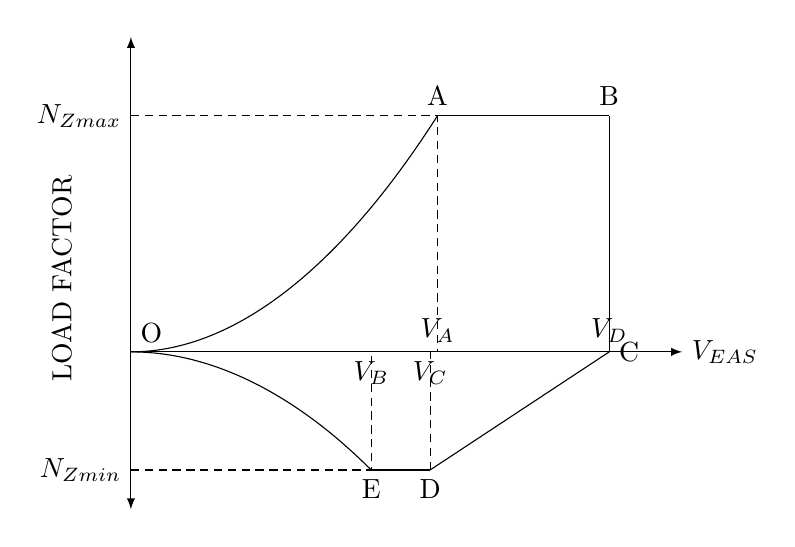
\begin{tikzpicture}
\coordinate (O) at (0, 0);

\begin{scope}[-latex]
\draw (O)--(7, 0)node[right]{$V_{EAS}$};
\draw (O)--(0, 4)node[left]{};
\draw (O)--(0, -2)node[left]{};
\end{scope}

\draw [densely dashed] (0, 3)node[left]
{$N_{Zmax}$}--(3.895, 3)node[above]
{A}--(3.895, 0)node[above]{$V_A$};

\draw [densely dashed] 
(6.075, 3)node[above]
{B}--(6.075, 0)node[above]{$V_D$};

\draw(3.895, 3)--(6.075, 3);
\draw(6.075,3)--(6.075,0);
\draw (6.075,0)node[right]{C};

\draw [densely dashed] (0, -1.5)node[left]{$N_{Zmin}$}--(3.052, -1.5)node[below]
{E}--(3.052, 0)node[below]{$V_B$};

\draw [densely dashed]
(3.8, -1.5)node[below]
{D}--(3.8, 0)node[below]{$V_C$};

\draw(0,0)node[above right]{O
};
\draw(3.052,-1.5)--(3.8,-1.5);
\draw(3.8,-1.5)--(6.075,0);

\draw (0,0) parabola (3.895,3);
\draw (0,0) parabola (3.052, -1.5);
\node[label={[label distance=0.5cm,text depth=-1ex,rotate=90]right:LOAD FACTOR}]
at (-1,-1) {};

\end{tikzpicture}
\caption{V-n線図}
\label{fig:v-n}
\end{figure}
